\subsection{Content Server} \label{section:counter-replace-server}
Moving the license verification to a server is one approach to fight the shortcomings of the license verification libraries.
By introducing service managed accounts, the user has to login on a server in order retrieve content for the application.
Since the applications logic is on a server, Lucky Patcher is not able to manipulate the verification logic.
\begin{figure}[h]
    \centering
    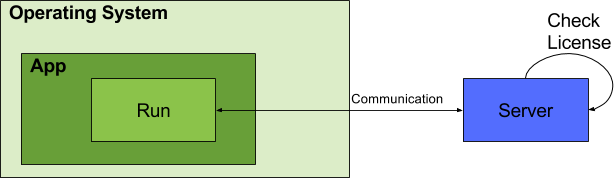
\includegraphics[width=0.8\textwidth]{data/contentServer.png}
    \caption{Abstraction of an application and a content server}
    \label{fig:contentServer}
\end{figure}
The implementation can be described with the application Spotify \cite{spotify} as a reference.
Instead of using local license verification, the user has to enter his credentials, which are send to the server.
In case the credentials are valid, the user is logged into the application.
The content, music in this case, is no longer on the phone itself, but streamed from the server.
In case a attackers circumvent the user verification, they are facing a second layer of security since it is not possible to access the content on the server without a verified account.
Thus attacks on the applications are not simple anymore.
\newline
This would be a perfect solution if there were not downsides as well.
The first problem is that this model cannot be applied universally.
This means that it must be possible to extract parts of the application's logic and implement them on a server.
The second one are the additional resources needed.
When realizing parts of the application on a server, not only knowledge and money is needed for the server, an additional application for the server has to be created as well.
Not every developer can handle this additional workload.
The third problem is the resulting always online necessaty which limits the freedom of users and might make the application less accepted.
\newline
Nevertheless, in case this implementation can be realized, it is an almost safe solution.
As a byproduct, the protection of the \gls{ip} can be achieved as well by moving the core algorithm, when possible, to server.
This prevents attackers not from only using the application for free, but also from reconstructing the the core functionality and implementing it somewhere else and thus the application offers less value to attackers.
